After looking at feature trends and fingerprintability of major
browsers, one interesting question to attempt to answer is this: If
browser fingerprinting is becoming easier over time because Firefox
and Chrome are, in general, becoming more ``bloated'' with features,
does this mean that these browsers are also becoming less secure over
time?  After all, the common folk wisdom is that if a software is more
bloated, it offers more vulnerabilities and a larger attack surface to
launch attacks against (e.g.,~\cite{Bloating}). In this section, we
attempt to answer if there is a direct link between the number of
features a specific browser offers, and the number of vulnerabilities
that have been reported for that browser version.

To answer this question, we extracted the CVE reports for Chrome and
Firefox from 2016 to 2020 as discussed in the methodology section. We
parsed these reports automatically, and generated CVEs that are
related to Google Chrome and Mozilla Firefox for the versions we were
interested in. For Chrome, most CVEs were affecting Google Chrome
49.0.2623 which had 919 reported CVEs. In contrast, Chrome
81.0.4044.129 had the least number of CVEs -- hence, making it the
most secure Google Chrome version. In contrast, for Firefox, 589 CVEs
were reported for Firefox 45 which made it the most vulnerable Firefox
browser in our study. Compared to Firefox 45, Firefox 75 was the most
secure Firefox version in our study with only 11 CVEs. Detailed
information about the number of CVEs reported per browser version is
available in Figures \ref{fig:firefox-vuln} and \ref{fig:chrome-vuln}.

% Jordan added: framing the issue of vulnerabilities vs. fingerprinting
We note a subtle but important distinction between the kinds of
vulnerabilities tracked in the CVE database and privacy concerns like
browser fingerprintability. The MITRE CVE database web
portal~\footnotemark defines a \textit{vulnerability} as ``[a] flaw in a
software, firmware, hardware, or service component resulting from a
weakness that can be exploited, causing a negative impact to the
confidentiality, integrity, or availability of an impacted component or
components.''
\footnotetext{\url{https://cve.mitre.org/about/terminology.html\#vulnerability}}
CVE entries thus track unambiguous flaws in system design or
implementation, such as buffer overflows or privilege escalation
vulnerabilities.  They do not typically cover more ambiguous privacy
concerns that involve the abuse of otherwise-properly implemented system
features. For example, while widespread consensus found the Battery
Status~\cite{olejnik2017battery} browser API to be an egrigious vector
for user fingerprinting, and conscientious browser vendors subsequently
deprecated it, there is no mention of the Battery Status API in the CVE
database. It is thus possible for a system to be decreasing in
practically exploitable vulnerabilities per the CVE database while
increasing in general fingerprintability or other privacy-related
issues.

\begin{figure}[ht]
    \centering
    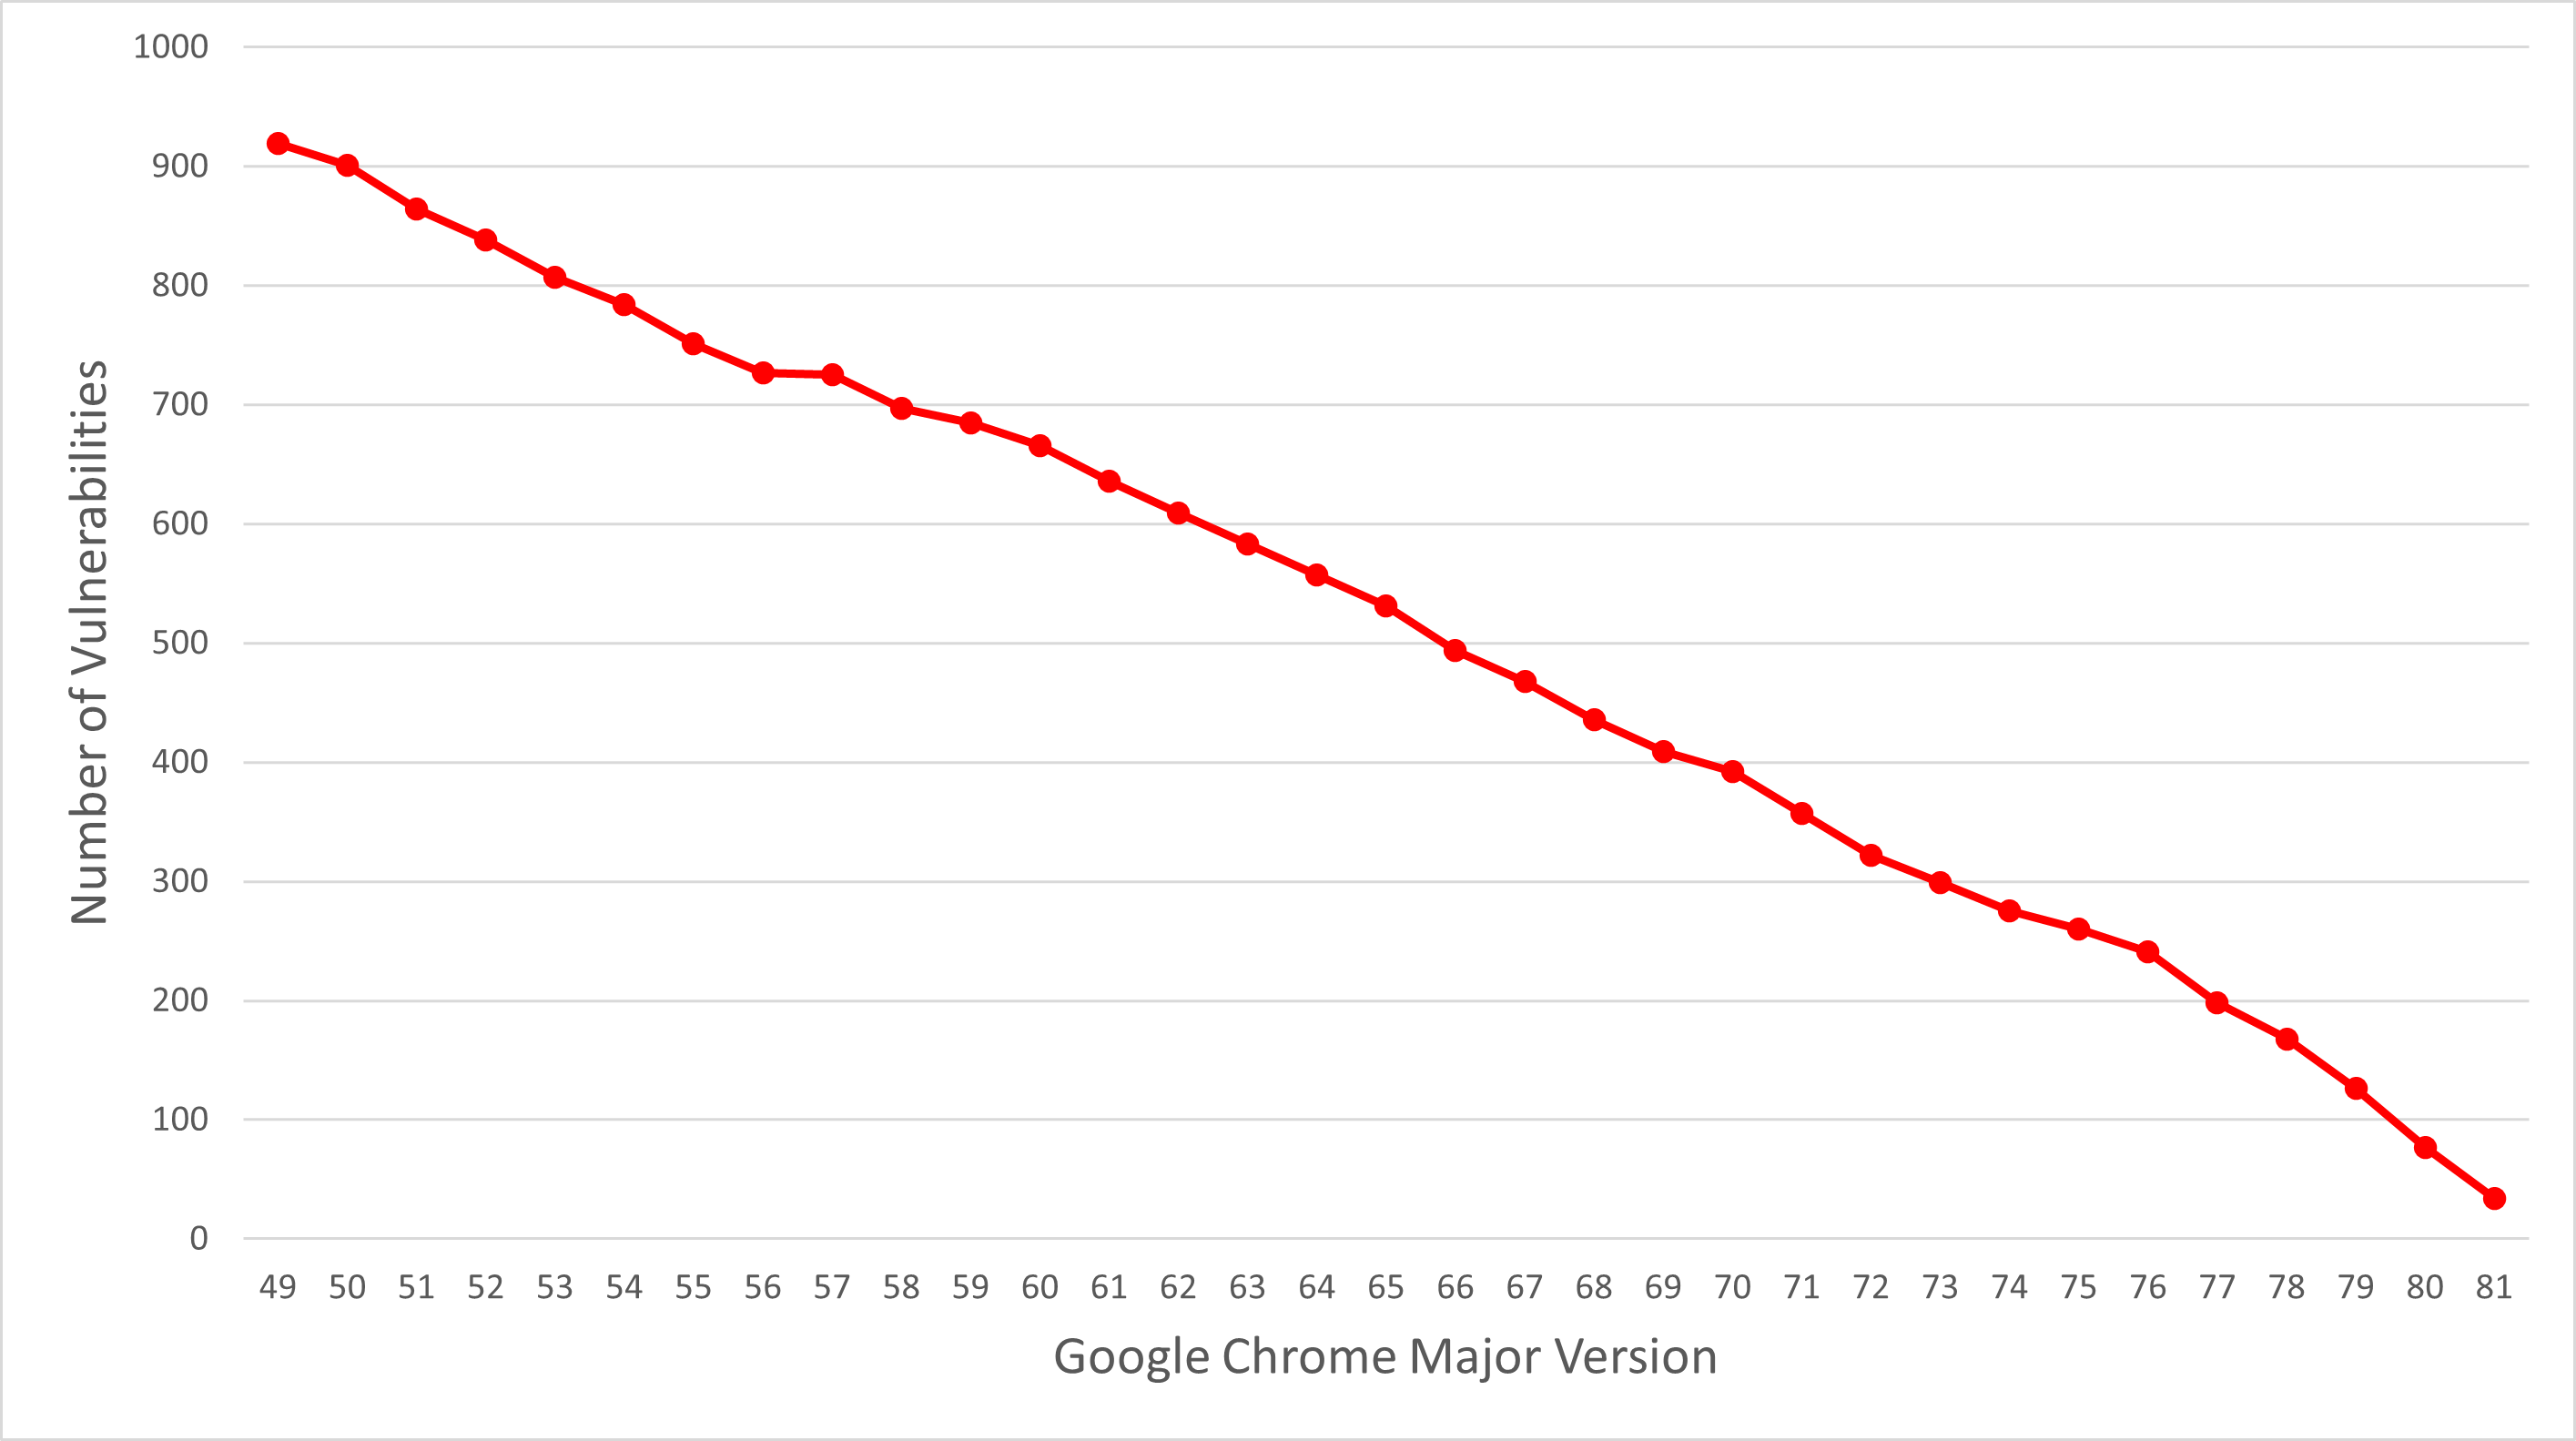
\includegraphics[width=\columnwidth]{figures/Chrome-Vulnerabilities.png}
    \caption{Google Chrome vulnerabilities per version.}
    \label{fig:chrome-vuln}
\end{figure}

\begin{figure}[ht]
    \centering
    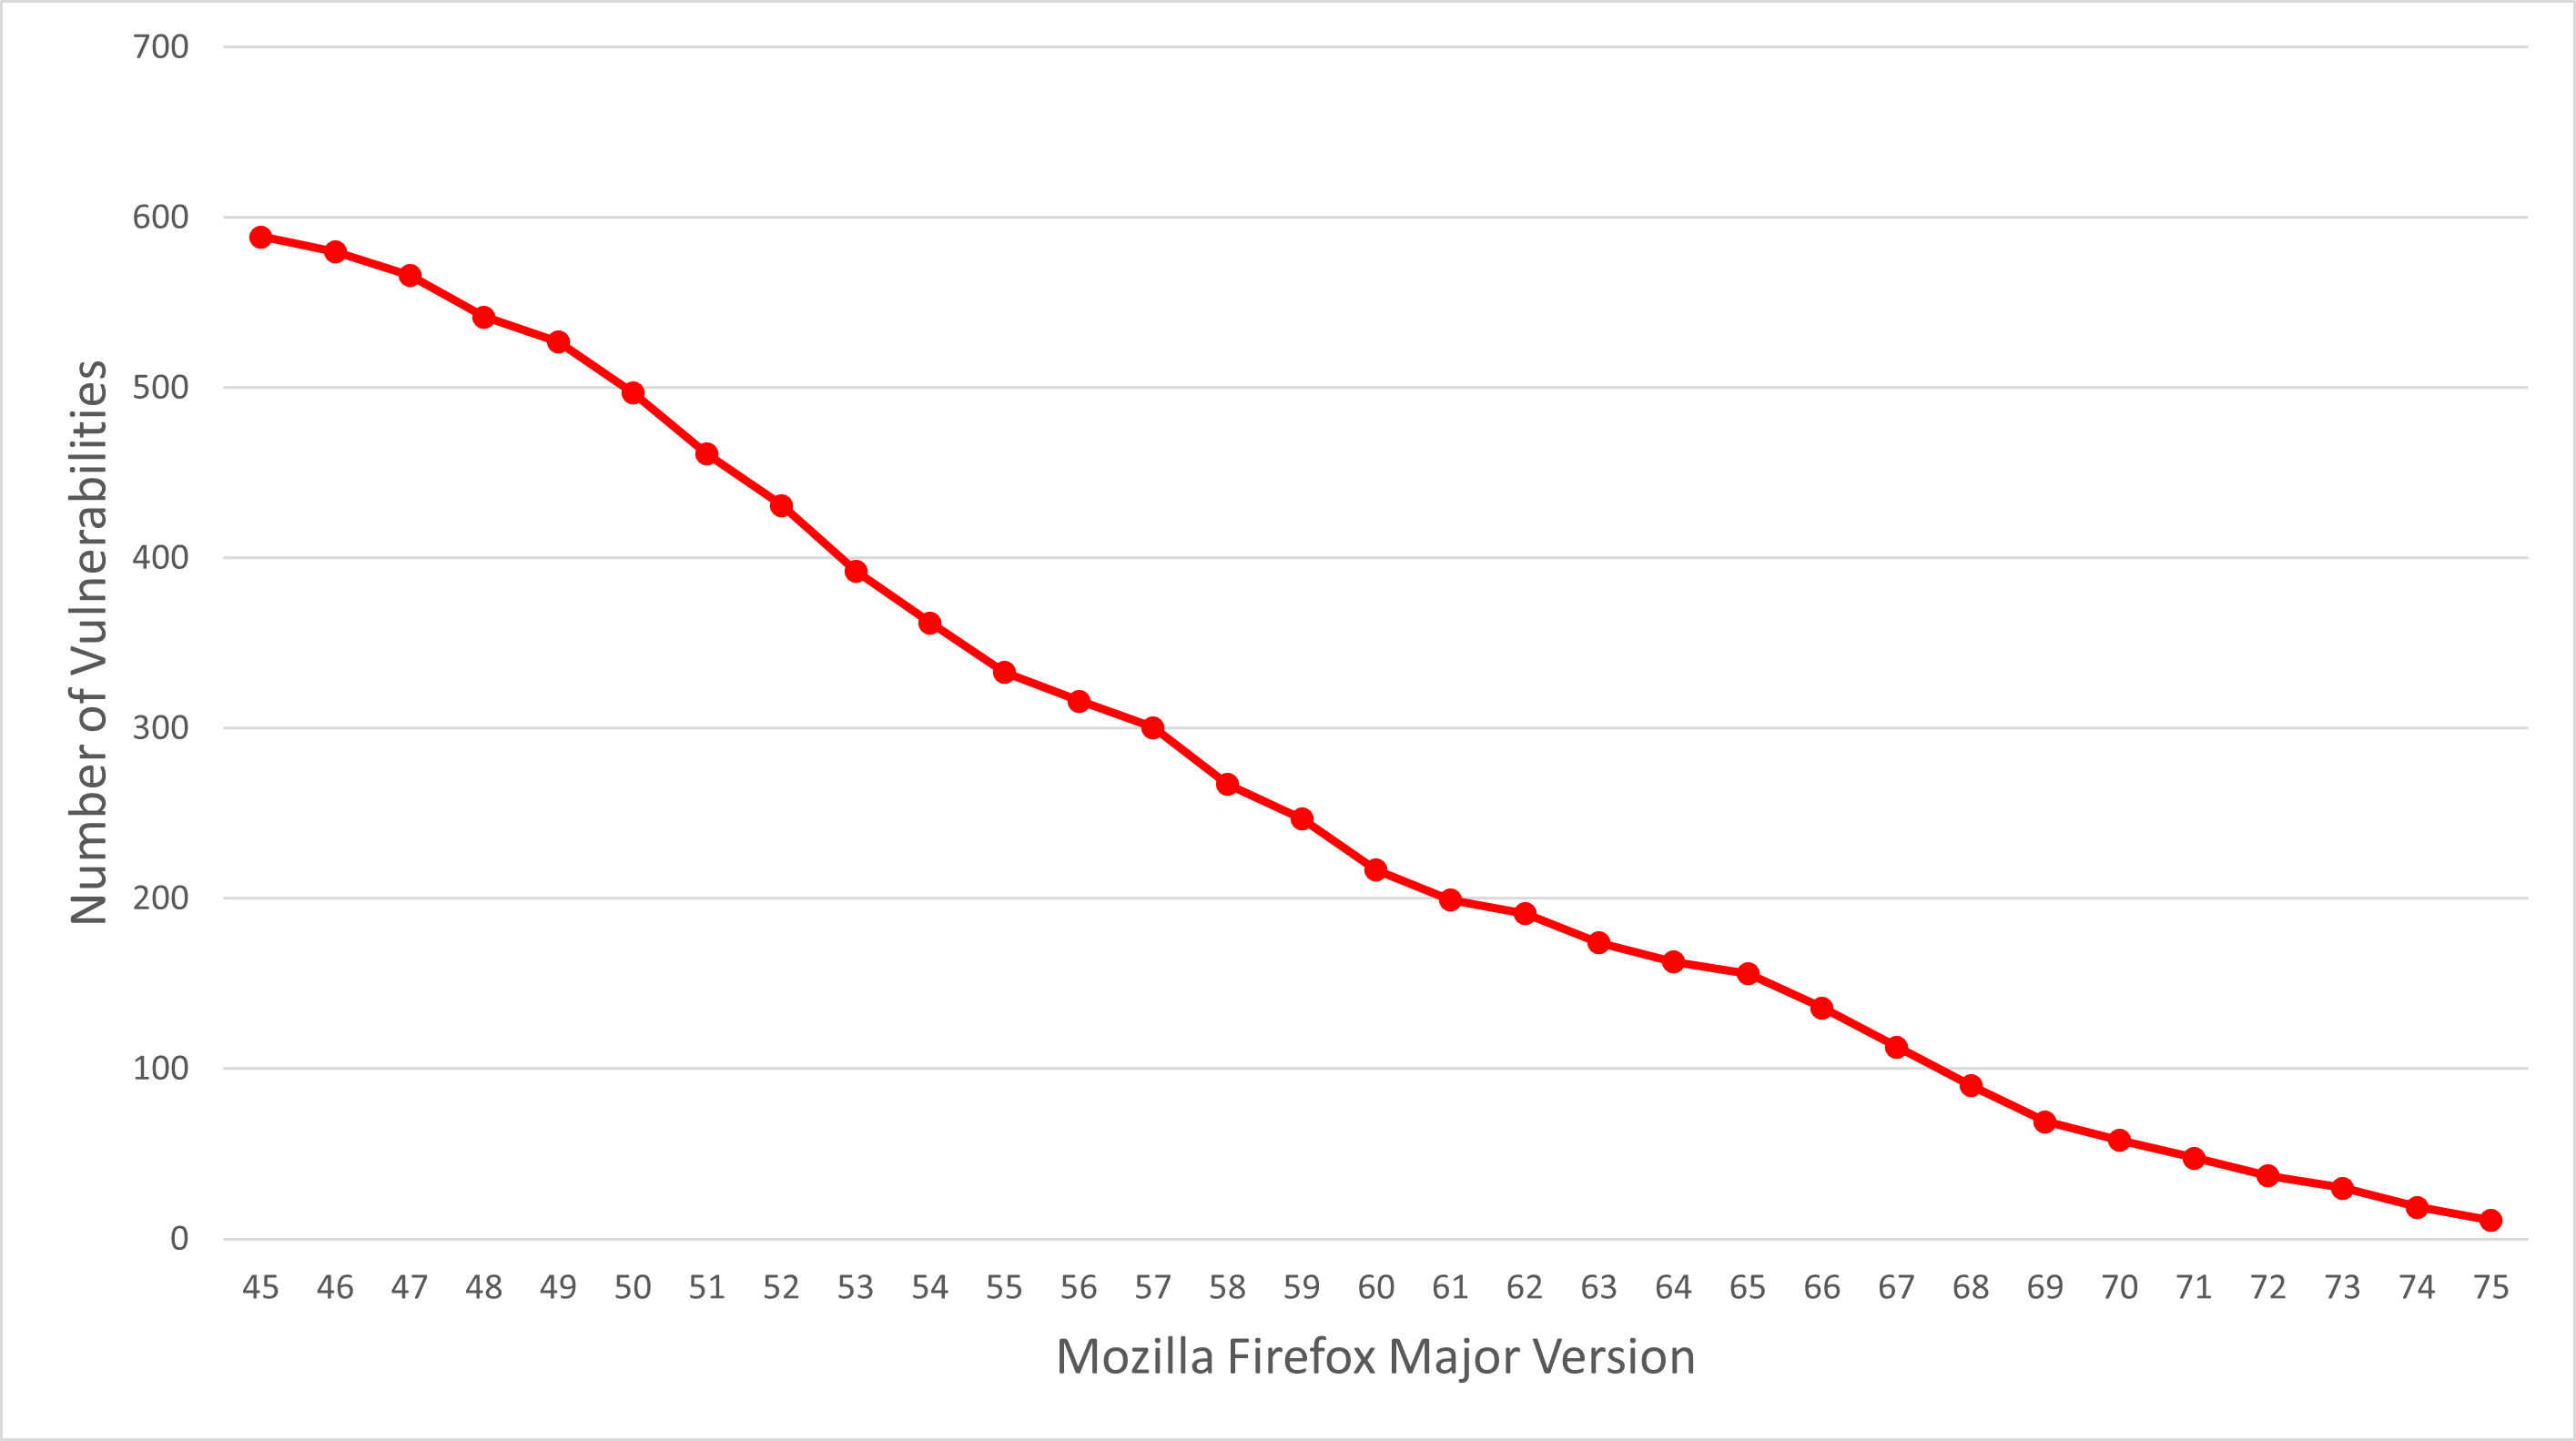
\includegraphics[width=\columnwidth]{figures/Firefox-Vulnerabilities.png}
    \caption{Mozilla Firefox vulnerabilities per version.}
    \label{fig:firefox-vuln}
\end{figure}


% Jordan updated/extended: multiple factors possible for CVE decline
If we compare CVE date per browser version with the feature trends we
reported in Figure \ref{fig:featuretrends}, it is evident that the
increase in the number of reported vulnerabilities does not correlate
with the increase in the number of supported browser features.  We
conjecture that a number of factors are interacting to cause this
counter-intuitive result.  First, older browser versions have existed,
and thus been under attack by fuzzers and other vulnerability research
efforts, for longer than newer versions. This simple fact should
naturally result in more reported vulnerabilities for older versions,
though the aggressive update policies of all modern browsers make the
practical threat posed by old, vulnerable browser versions very low for
typical users.  Second, browser vendors are investing heavily in making
their browser codebases more robust and
secure~\cite{FirefoxCrashes,ChromeSecure}, making it very likely that
the downward trend is not \textbf{just} an artifact of time-under-attack
but an actual hardening of codebases.  Finally, aggressive updates and
general hardening of browsers produce perverse economic incentives for
vulnerability researchers as the black market prices of practical
browser exploits rise to dizzying
levels.~\cite{TODO-recent-exploit-pricing} In conclusion, while the
general intuition that code ``bloating'' leads to more security problems
may be correct in general, this assumption does not appear to hold true
for modern browsers.

